% Indicate the main file. Must go at the beginning of the file.
% !TEX root = ../main.tex

%%%%%%%%%%%%%%%%%%%%%%%%%%%%%%%%%%%%%%%%%%%%%%%%%%%%%%%%%%%%%%%%%%%%%%%%%%%%%%%%
% 02_methods
%%%%%%%%%%%%%%%%%%%%%%%%%%%%%%%%%%%%%%%%%%%%%%%%%%%%%%%%%%%%%%%%%%%%%%%%%%%%%%%%

\section{Methods}
\label{methods}

\subsection{Data}%%%%%%%%%%%%%%%%%%%%%%%%%%%%%%%%%%%%%%%%%%%%%%%%%%%%%%%%%%%%%%%

The used data for this project is the SwissImage RS \autocite{SWISSIMAGERS} data from the Swiss Federal Office of Topography (swisstopo).
It is a raster dataset with a resolution of 0.1m containing four bands: RGB and NIR.
In order to cover the area of interest (AOI) 6 tiles of the dataset are needed.
Over this large AOI there are three areas labeled with the corresponding landcover categories.
This labeled data was provided by a team of researchers from the ZHAW. The three
areas are distributed over a residential area (83487m\textsuperscript{2}),
qn industrial area (132642m\textsuperscript{2}) and a rural area (82740m\textsuperscript{2}) \autoref{fig:category_areas}.
There are 10 different landcover categories in total shown in \autoref{fig:landcover_categories}.

\begin{figure}[H]
    \centering
    \captionsetup{width=0.8\linewidth}
    \includegraphics[width=\linewidth]{figures/category_areas.png}
    \caption{The three areas with the corresponding landcover categories.}
    \label{fig:category_areas}
\end{figure}

\begin{figure}[H]
    \centering
    \captionsetup{width=0.8\linewidth}
    \includegraphics[scale=0.6]{figures/area_by_category.pdf}
    \caption{Available data by label, colored by the area.}
    \label{fig:landcover_categories}
\end{figure}

\subsection{Data Processing}%%%%%%%%%%%%%%%%%%%%%%%%%%%%%%%%%%%%%%%%%%%%%%%%%%%%

In a first step the data was processed using ArcGIS Pro. The process included a few steps implemented as
a model \autoref{fig:processing_model}. The 6 tiles where mosaicked together and the area of interest 
was clipped. The landcover categories where transformed into a raster dataset and added as additional
band as well as an extra mask band constructed for orientation purposes. To get an overview of the
available data refer to \autoref{fig:aoi_labeled}. The data was then exported as a GeoTIFF file.
In order to use the data in a neural network an additional step was necessary. Using a custom Python script,
the data was transformed into Zarr format. This format is a chunked, compressed, N-dimensional array
storage format with multi-scale support. This allows for lazy loading and therefore for a more memory
efficient data access during training.

\begin{figure}[H]
    \centering
    \captionsetup{width=0.8\linewidth}
    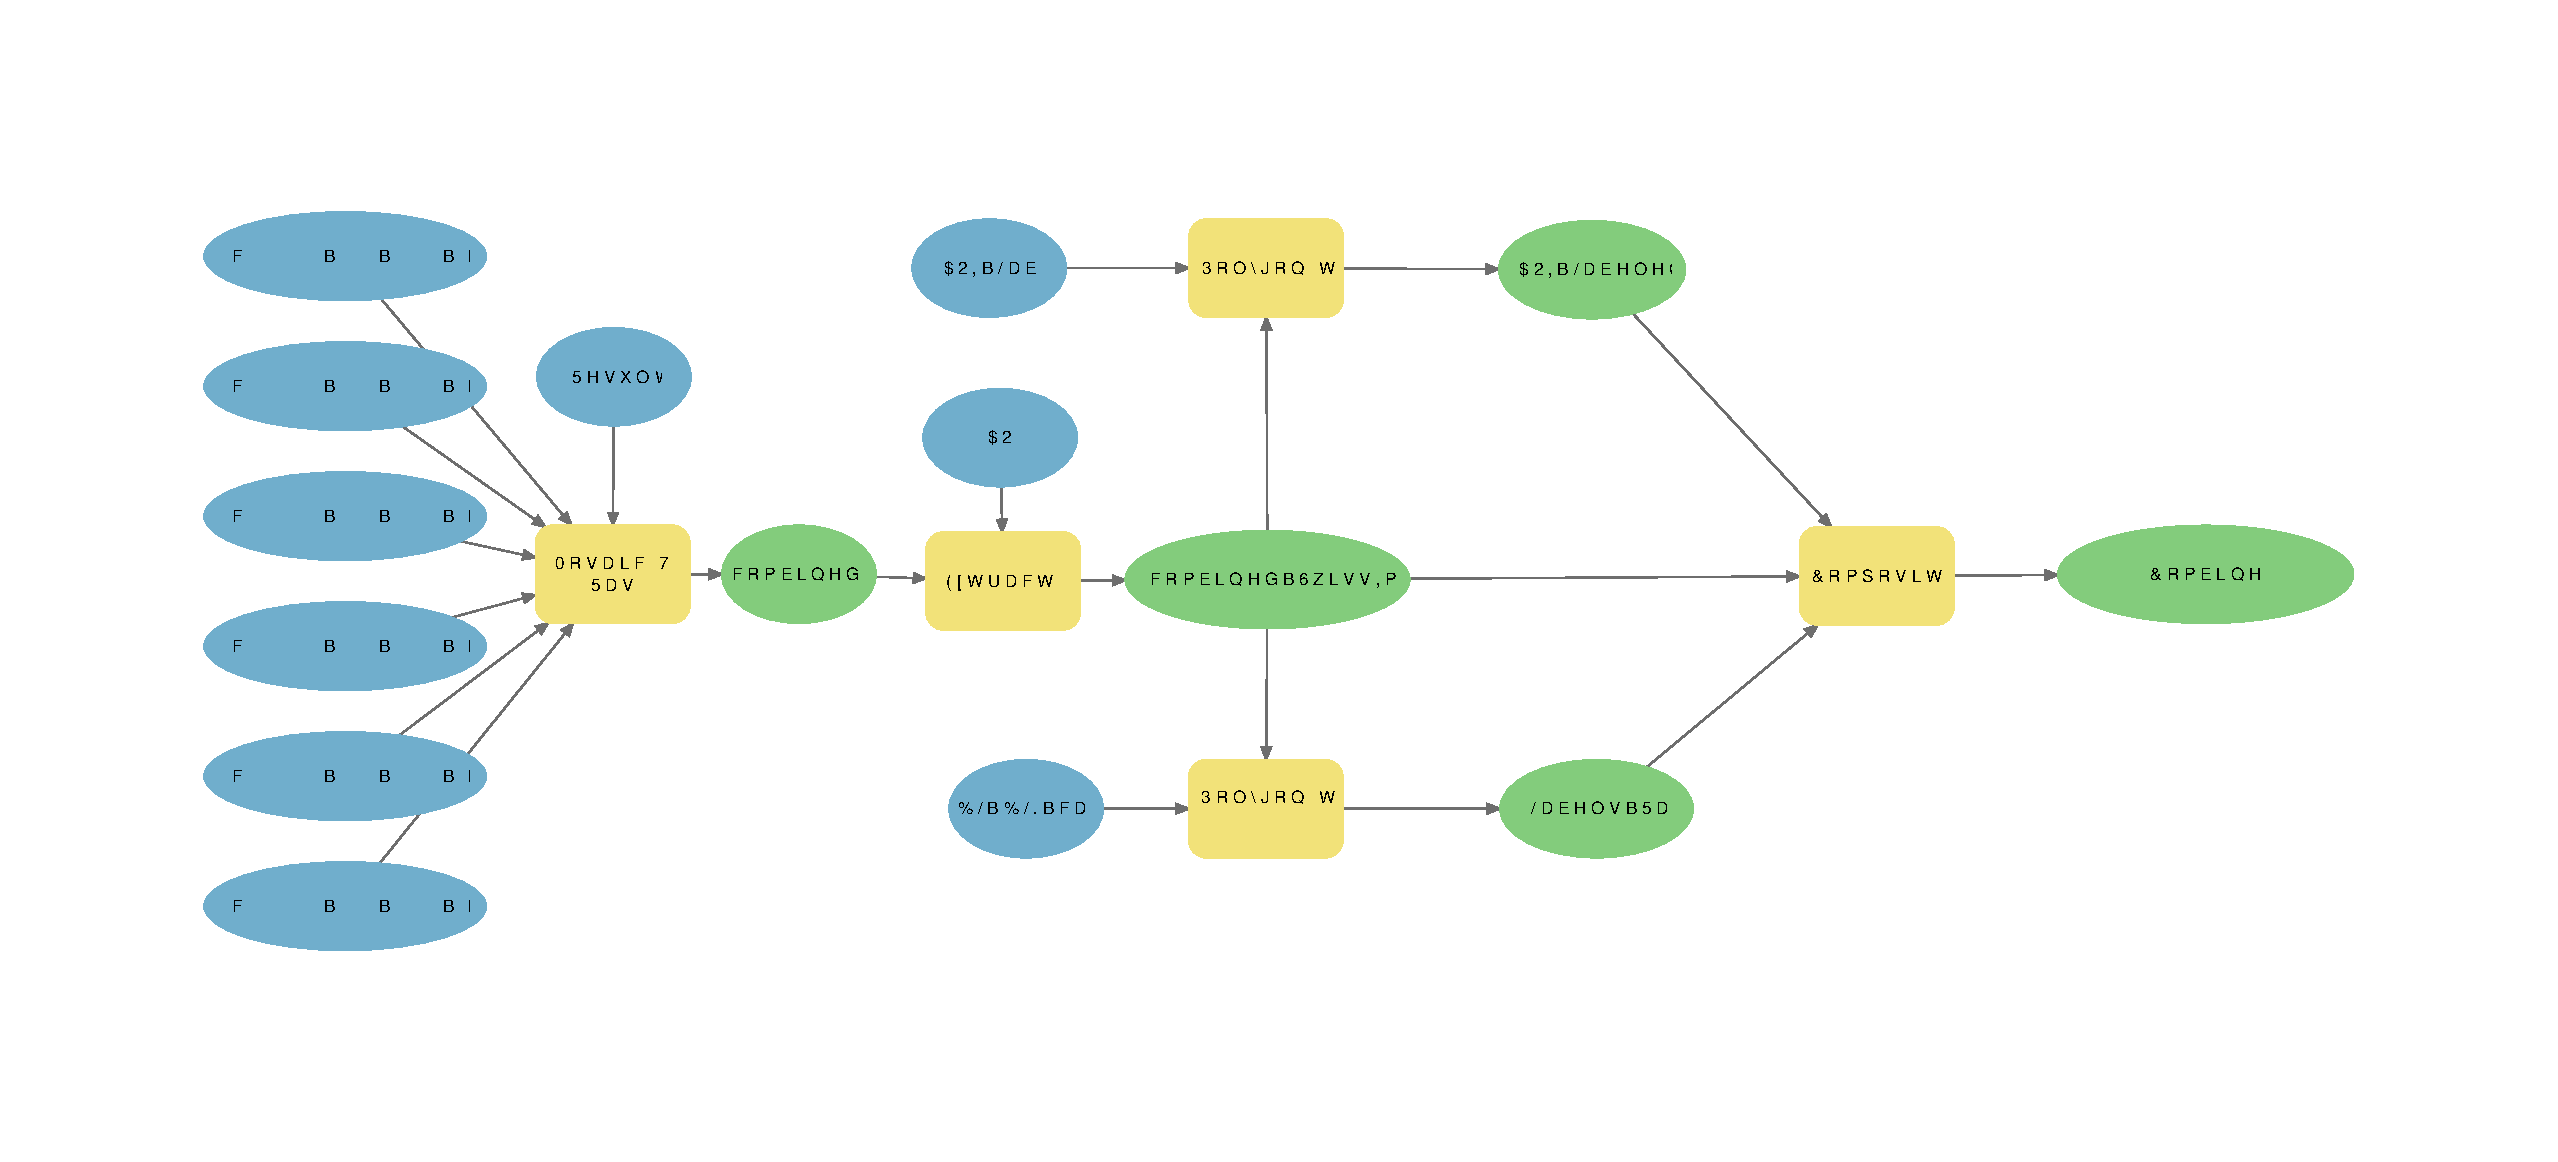
\includegraphics[width=\linewidth]{figures/Model.pdf}
    \caption{The ArcGis model used for preprocessing the data.}
    \label{fig:processing_model}
\end{figure}

\begin{figure}[H]
    \centering
    \captionsetup{width=0.8\linewidth}
    \includegraphics[scale=0.6]{figures/AOI_Labeled.png}
    \caption{The area of interest with the three labeled areas.}
    \label{fig:aoi_labeled}
\end{figure}



\subsection{Data Loader and Augmentation}%%%%%%%%%%%%%%%%%%%%%%%%%%%%%%%%%%%%%%%%

A custom DataLoader was implemented using PyTorch. The DataLoader is designed to index the available data
depending on the cutout size. It handles the data augmentation on the fly, during the training.
For the data augmentation a parent class BaseAugmentor was implemented from which the different augmenters inherit. The implemented augmentors -
refer to \autoref{tab:augmentors} - are then chained into a object of the class AugmentorChain
which is than used in the DataLoader.

\begin{table}[H]
    \centering
    \begin{tabular}{|l|l|}
        \hline
        \textbf{Augmentor} & \textbf{Description} \\
        \hline
        FlipAugmentor & Randomly flips the image vertically, horizontally or not at all \\
        RotateAugmentor & Randomly rotates the image 0, 90, 180 or 270° \\
        PixelNoiseAugmentor & Adds random noise to the image (parameter: scale) \\
        ChannelNoiseAugmentor & Adds random noise to the channels (parameter: scale) \\
        \hline
    \end{tabular}
    \caption{Implemented augmentors}
    \label{tab:augmentors}
\end{table}
